% chktex-file 8

\tolerance=10000 Η εκτεταμένη πραγματικότητα (Extended Reality - XR) αποτελεί μια ιδιαιτέρως ευρεία έννοια, η οποία χρησιμοποιήθηκε πρώτη φορά το 1991 από τους Steve Mann και Charles Wyckoff, κατά την προσπάθεια κατασκευής συσκευών εικονικής/επαυξημένης πραγματικότητας~\cite{mann_2023_fundamentals}\cite{mann_1991_extended}. Αποτελεί <<ομπρέλα>> εννοιών και περιλαμβάνει τις έννοιες της Εικονικής (Virtual Reality - VR, \hyperref[subsec:mixedReality]{Κεφάλαιο~\ref*{subsec:mixedReality}}), της Επαυξημένης (Augmented Reality - AR, \hyperref[subsec:augmentedReality]{Κεφάλαιο~\ref*{subsec:augmentedReality}}) και της Μικτής Πραγματικότητας (Mixed Reality - MR, \hyperref[subsec:mixedReality]{Κεφάλαιο~\ref*{subsec:mixedReality}})~\cite{milgram_1994_augmented}. To 1994, οι Paul Milgram και Fumio Kishino όρισαν ένα συνεχές μεταξύ πραγματικού και εικονικού κόσμου (\hyperref[fig:rv_continuum]{\schema~\ref*{fig:rv_continuum}}). Αυτοί οι δύο κόσμοι αποτελούν τα άκρα της κλίμακας και μεταξύ αυτών υπάρχουν οι έννοιες της επαυξημένης και μικτής πραγματικότητας, καθώς και της επαυξημένης εικονικότητας.
\begin{figure}[!h]
    \centering
    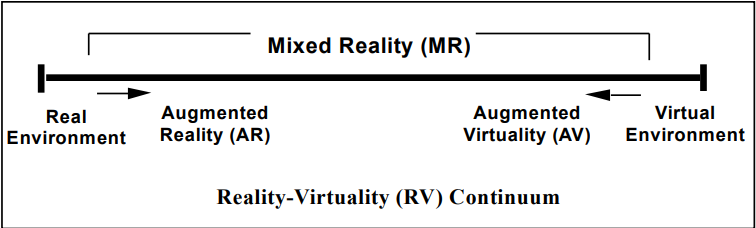
\includegraphics[width=120mm]{images/rv_continuum.png}
    \caption{Κλίμακα Πραγματικού Κόσμου - Εικονικού Κόσμου~\cite{milgram_1994_augmented}}\label{fig:rv_continuum}
\end{figure}

\subsection{Εικονική Πραγματικότητα}\label{subsec:virtualReality}
Η εικονική πραγματικότητα αποτελεί μια προσομοίωση, η οποία εντάσσει τον χρήστη σε έναν εικονικό κόσμο, κατασκευασμένος από υπολογιστή, διεγείροντας αισθήσεις όπως η όραση (μπορεί να δει τον κόσμο αυτόν), η ακοή (μπορεί να ακούσει ήχους που προέρχονται από τον κόσμο αυτόν) και η αφή (μπορεί να αντιληφθεί την επαφή με εικονικά αντικείμενα λαμβάνοντας απτική ανάδραση~\cite{weiler_2023_phantom}\cite{perret_2018_touching}), δίνοντάς του την δυνατότητα να αλληλεπιδράσει με αυτόν~\cite{lowood_2018_virtual}. Τα ανωτέρω επιτυγχάνονται με χρήση ειδικών συσκευών, όπως είναι τα γυαλιά εικονικής πραγματικότητας (VR headsets), τα οποία είτε ενσωματώνουν ειδικούς αισθητήρες με σκοπό να ανιχνεύσουν την κίνηση του κεφαλιού, είτε η ανίχνευση αυτή γίνεται με χρήση εξωτερικών αισθητήρων, που τοποθετούνται σε διάφορα σημεία στον περιβάλλοντα χώρο. Για την ανίχνευση της κίνησης των χεριών, που επιτρέπουν και την αλληλεπίδραση με εικονικά αντικείμενα, απαιτείται η χρήση χειριστηρίων. Παραδείγματα τέτοιων συσκευών αποτελούν το Meta Quest (\hyperref[fig:meta_quest_3]{\schema~\ref*{fig:meta_quest_3}}) και το Valve Index. Η VR τεχνολογία έχει εισβάλει πλέον και στην καθημερινότητα του μέσου χρήστη βρίσκοντας εφαρμογή σε ποικίλους τομείς:
\begin{itemize}
    \item Στην ψυχαγωγία και στη διασκέδαση, μέσω των βιντεοπαιχνιδιών που έχουν αναπτυχθεί, την δυνατότητα παρακολούθησης πραγματικών αθλητικών αγώνων, καθώς και εικονικών ξεναγήσεων σε χώρους πολιτιστικού ενδιαφέροντος~\cite{loeffler_1993_distributed}\cite{meta_2022_xtadium}\cite{ansari_2021_implementing}
    \item Στην εκπαίδευση, προσφέροντας έναν εναλλακτικό και διαδραστικό τρόπο εκμάθησης~\cite{hamad_2022_how}\cite{kavanagh_2017_a}\cite{freina_2015_a}
    \item Στην ιατρική, με σκοπό την εκπαίδευση και προετοιμασία ιατρών, καθώς και για να προσφέρει βοήθεια σε ασθενείς~\cite{chirico_2015_virtual}\cite{hamad_2022_how}\cite{snoswell_2019_immersive}\cite{gerup_2020_augmented}
\end{itemize}
\begin{figure}[!h]
    \centering
    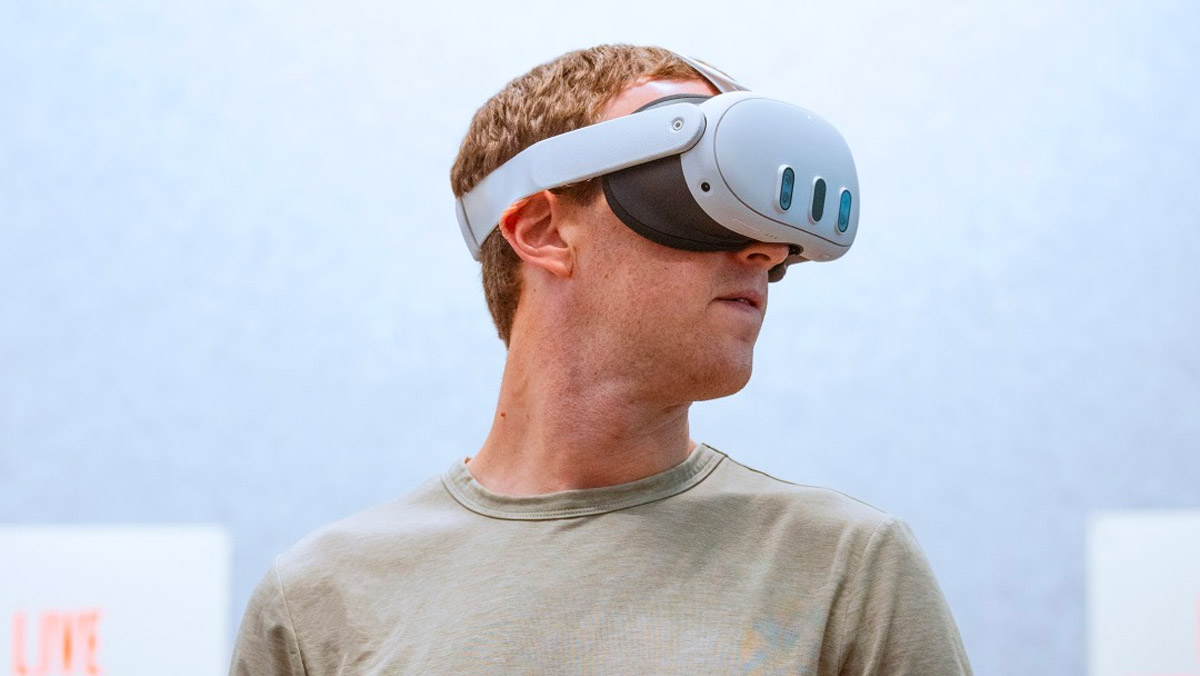
\includegraphics[width=90mm]{images/meta_quest_3.jpg}
    \caption{Χρήστης φορά τα γυαλιά εικονικής πραγματικότητας Meta Quest 3}\label{fig:meta_quest_3}
\end{figure}

\subsection{Επαυξημένη Πραγματικότητα}\label{subsec:augmentedReality}
Η επαυξημένη πραγματικότητα αποτελεί μια τεχνολογία, η οποία <<ενισχύει>> τον πραγματικό κόσμο, ενσωματώνοντας τεχνητά δημιουργημένα, από υπολογιστή, στοιχεία (εικονικά αντικείμενα, ήχους) σε αυτόν. Τα στοιχεία αυτά βρίσκονται εντός ενός <<στρώματος>> (layer), το οποίο τοποθετείται <<πάνω>> από τον πραγματικό κόσμο, ο οποίος μπορεί να είναι μια φωτογραφία, ένα βίντεο ή ένα βίντεο πραγματικού χρόνου~\cite{hosch_2020_augmented}\cite{carmigniani_2011_augmented}. Λόγω της εξέλιξης των επεξεργαστών και της απλότητας της τεχνολογίας (σε σχέση με την εικονική πραγματικότητα), ένας χρήστη μπορεί να βιώσει την εμπειρία της επαυξημένης πραγματικότητας χρησιμοποιώντας μια απλή, έξυπνη κινητή συσκευή (smartphone)~\cite{ko_2013_usability}. Παράλληλα, είναι διαθέσιμα και γυαλιά επαυξημένης πραγματικότητας (AR headsets), όπως είναι τα Xreal Air AR Glasses και Magic Leap 2.

Η επαυξημένη πραγματικότητα βρίσκει εφαρμογή σε παρόμοιους τομείς με αυτούς της εικονικής πραγματικότητας:
\begin{itemize}
    \item Στην εκπαίδευση~\cite{wu_2013_current}\cite{lee_2012_augmented}
    \item Στον εργασιακό χώρο, αποτελώντας ένα επιπλέον εργαλείο για τον εργαζόμενο με σκοπό να διευκολύνει το έργο και να βελτιώσει την απόδοσή του~\cite{kim_2016_augmented}\cite{funk_2017_working}\cite{pereira_2023_augmented}
    \item Στην υγεία~\cite{klinker_2019_digital}\cite{zhu_2015_design}\cite{gerup_2020_augmented}\cite{solbiati_2020_augmented}
    \item Στην ψυχαγωγία~\cite{hung_2021_a}
    \item Στον τουρισμό, παρέχοντας ξεναγήσεις, όπου ο χρήστης μπορεί να μάθει περισσότερες πληροφορίες για μνημεία απλά στοχεύοντας την κάμερα του κινητού του σε αυτά~\cite{yovcheva_2012_smartphone}\cite{kounavis_2012_enhancing}
\end{itemize} 

\subsection{Μικτή Πραγματικότητα}\label{subsec:mixedReality}
Η `μικτή πραγματικότητα' αποτελεί μια έννοια, η οποία, μέχρι και πρόσφατα, δεν έχει προσδιοριστεί ξεκαθάρα και επιδέχεται πληθώρα ορισμών, οι οποίοι, ωστόσο, διαθέτουν μια κοινή βάση~\cite{speicher_2019_what}. Βάση του ορισμού που δόθηκε από τους Milgram και Kishino με το Συνεχές Πραγματικού-Εικονικού Κόσμου (\hyperref[fig:rv_continuum]{\schema~\ref*{fig:rv_continuum}}), η μικτή πραγματικότητα αποτελεί οτιδήποτε ανήκει μεταξύ των δύο άκρων της κλίμακας, όντας η επαυξημένη πραγματικότητα και η επαυξημένη εικονικότητα. Με τον όρο επαυξημένη εικονικότητα εννοείται ένας εικονικός κόσμος, στον οποίο ενσωματώνονται πραγματικά αντικείμενα του περιβάλλοντα χώρου~\cite{milgram_1994_augmented}. Ορισμένοι ακόμη δημοφιλείς ορισμοί της μικτής πραγματικότητας είναι:
\begin{enumerate}
    \item Η μικτή πραγματικότητα αποτελεί συνώνυμο της επαυξημένης πραγματικότητας
    \item Η τεχνολογίας μικτής πραγματικότητας αποτελεί μια ενισχυμένη μορφή της τεχνολογίας επαυξημένης πραγματικότητας, όπου τα εικονικά αντικείμενα αλληλεπιδρούν με το πραγματικό περιβάλλον και τα αντικείμενα σε αυτόν
    \item Η μικτή πραγματικότητα αποτελεί συνδυασμός της επαυξημένης και της εικονικής πραγματικότητας, ενσωματώνοντας στοιχεία και από τις δύο τεχνολογίες
\end{enumerate}
Παράδειγμα συσκευών που αξιοποιούν την τεχνολογία μικτής πραγματικότητας αποτελούν τα Microsoft HoloLens, Apple Vision Pro και Meta Quest Pro.
Η μικτή πραγματικότητα βρίσκει και αυτή ευρεία εφαρμογή σε αρκετούς τομείς της σύγχρονης καθημερινότητας, όπως είναι η εκπαίδευση~\cite{knierim_2018_challenges}\cite{liu_2007_mixed}, η υγεία~\cite{chen_2017_recent}\cite{tepper_2017_mixed}, η αρχιτεκτονική~\cite{wang_2008_mixed}\cite{dunston_2005_mixed} κ.α.